\chapter{Elektronika}

\section{Podzespoły}
\label{sec:czesci}
\subsection{Mikrokontroler}
\label{sec:STM32}
W urządzeniu został wykorzystany mikrokontroler firmy STMicroelectronics STM32F407 Discovery ukazany na rysunku \ref{fig:STM32}. Moduł wyposażony jest w 32-bitowy rdzeń ARM Cortex M4F. Maksymalne taktowanie mikroprocesora to 168 MHz, oferuje 1 MB pamięci flash oraz 192 kB pamięci RAM. Dodatkowo moduł jest wyposażony w dedykowany programator ST-LINK/V2, który pozwala również na debuggowanie. Mikrokontroler oferuje wiele programowalnych wejść i wyjść, a w tym między innymi w trybie wejścia sygnału enkodera czy wyjścia sygnału PWM. Moduł można zasilać zarówna z 5V jak i 3,3V. Zapotrzebowanie prądowe mikrokontroler to maksymalnie około 40mA. Płytka wraz ze sterownikiem silnika zostały przymocowane do konstrukcji przy pomocy samodzielnie zaprojektowanego uchwytu. 

\begin{figure}
    \centering
    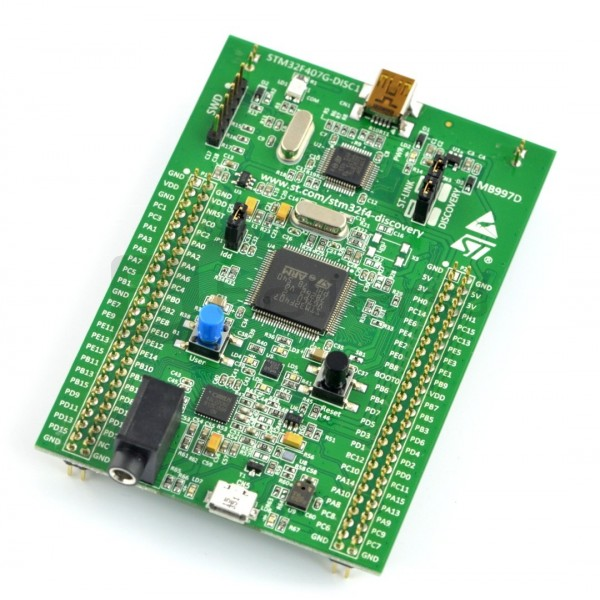
\includegraphics[scale=0.8]{praca_dyplomowa/figures/STM32F407.jpg}
    \caption{Mikrokontroler STM32F407 Discovery}
    \texttt{Źródło: botland.com.pl}
    \label{fig:STM32}
\end{figure}

\subsection{Enkoder}
Jako czujnik kąta odchylenia wahadła został wykorzystany enkoder DFRobot 400P/R, przedstawiony na rysunku \ref{fig:Enkoder}. Czujnik ma rozdzielczość 400 impulsów na każdy z 2 kanałów. Na wyjściach generowane są sygnały kwadraturowe, które są przesunięte w fazie względem siebie o 90\degree. W zależności od tego, na którym kanale najpierw pojawia się sygnał można rozróżnić kierunek obrotów. Przy zliczaniu zliczaniu wszystkich zboczy sygnałów maksymalna rozdzielczość wynosi 1600 impulsów na obrót z czego wynika, ze jeden impuls to odchylenie o 0,225\degree. Enkoder może być zasilany napięciem od 4,8V do 24V. Sygnały wyjściowe czujnika są generowane przez tranzystory NPN w układzie otwartego kolektora, przez co linie sygnałowe wymagają podciągnięcia przez rezystory do dodatniej linii zasilania (pull-up).

\begin{figure}
    \centering
    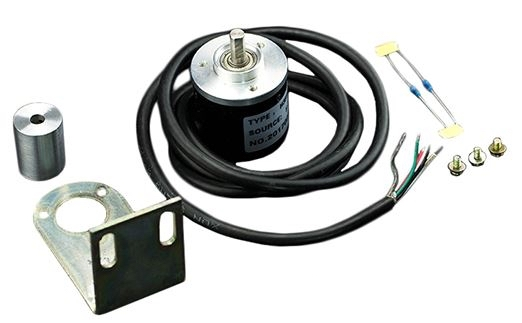
\includegraphics[scale=0.7]{praca_dyplomowa/figures/encoder.jpg}
    \caption{Enkoder DFRobot 400P/R}
    \texttt{Źródło: jsumo.com}
    \label{fig:Enkoder}
\end{figure}

\subsection{Silnik}
Do poruszania karetką został wykorzystany silnik prądu stałego Pololu 37Dx65L, ukazany na rysunku \ref{fig:Silnik}. Napięcie zasilania silnika to 12V, minimalny pobór prądu to 0,2A, a maksymalny przy zatrzymaniu wału 5,5A. Silnik wyposażony jest w przekładnię o przełożeniu 6,25:1, dzięki której osiąga 1600 RPM przy nominalnym napięciu, a moment obrotowy wynosi 3kg/cm, czyli 0,294Nm. Dodatkowo silnik posiada własny enkoder o rozdzielczości 16 impulsów na obrót na każdym kanale co maksymalnie daje 64 impulsy na pełny obrót. Enkoder silnik może być zasilany napięciem od 3,5V do 20V. 

\begin{figure}
    \centering
    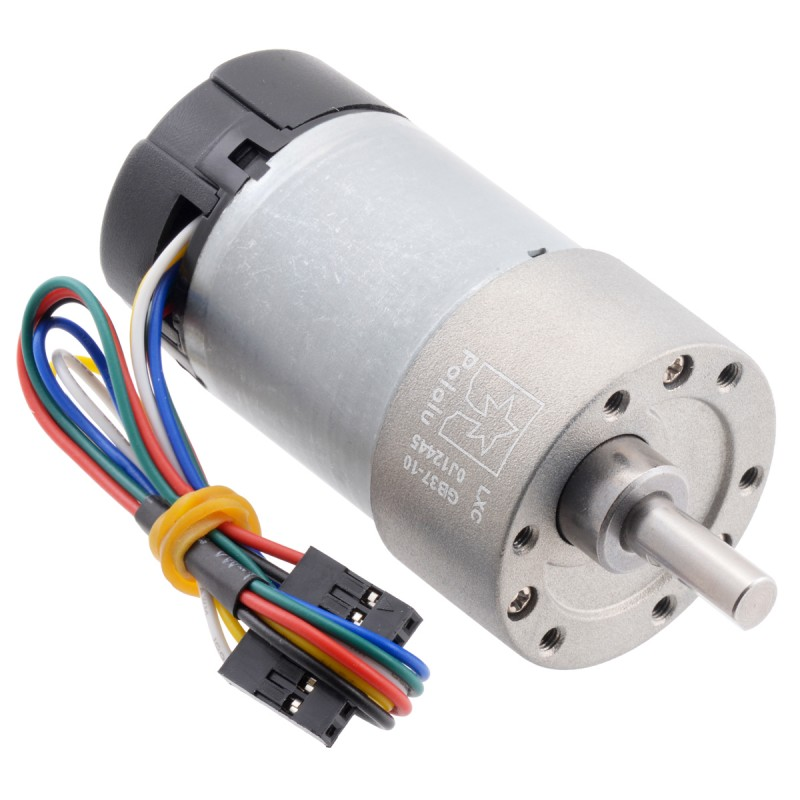
\includegraphics[scale=0.3]{praca_dyplomowa/figures/Pololu 37D.jpg}
    \caption{Silnik DC Pololu 37D}
    \texttt{Źródło: kamami.pl}
    \label{fig:Silnik}
\end{figure}

\subsection{Sterownik silnika}
Do sterowania silnikiem DC został wykorzystane moduł wyposażony w sterownik L298N, widoczny na rysunku \ref{fig:L298N}. Układ ten umożliwia sterowanie 2 silnikami dzięki dwóm osobnym kanałom. Napięcie zasilania silników może być dowolne z przedziału 4,8V do 46V, natomiast część logiczna wymaga zasilania napięciem 5V. Maksymalny prąd wyjściowy to 2A na każdy kanał, a dodatkowo kanały można połączyć ze sobą równolegle przez dwukrotnie zwiększy się wydajność prądowa. Maksymalna moc jaką potrzebuje sterownik to około 48W. Moduł, dzięki zastosowaniu mostka H, pozwala sterować silnikiem w różnych kierunkach, a także stosować szybkie lub wolne hamowanie. Prędkość obrotów silnika można regulować sygnałem PWM.

\begin{figure}
    \centering
    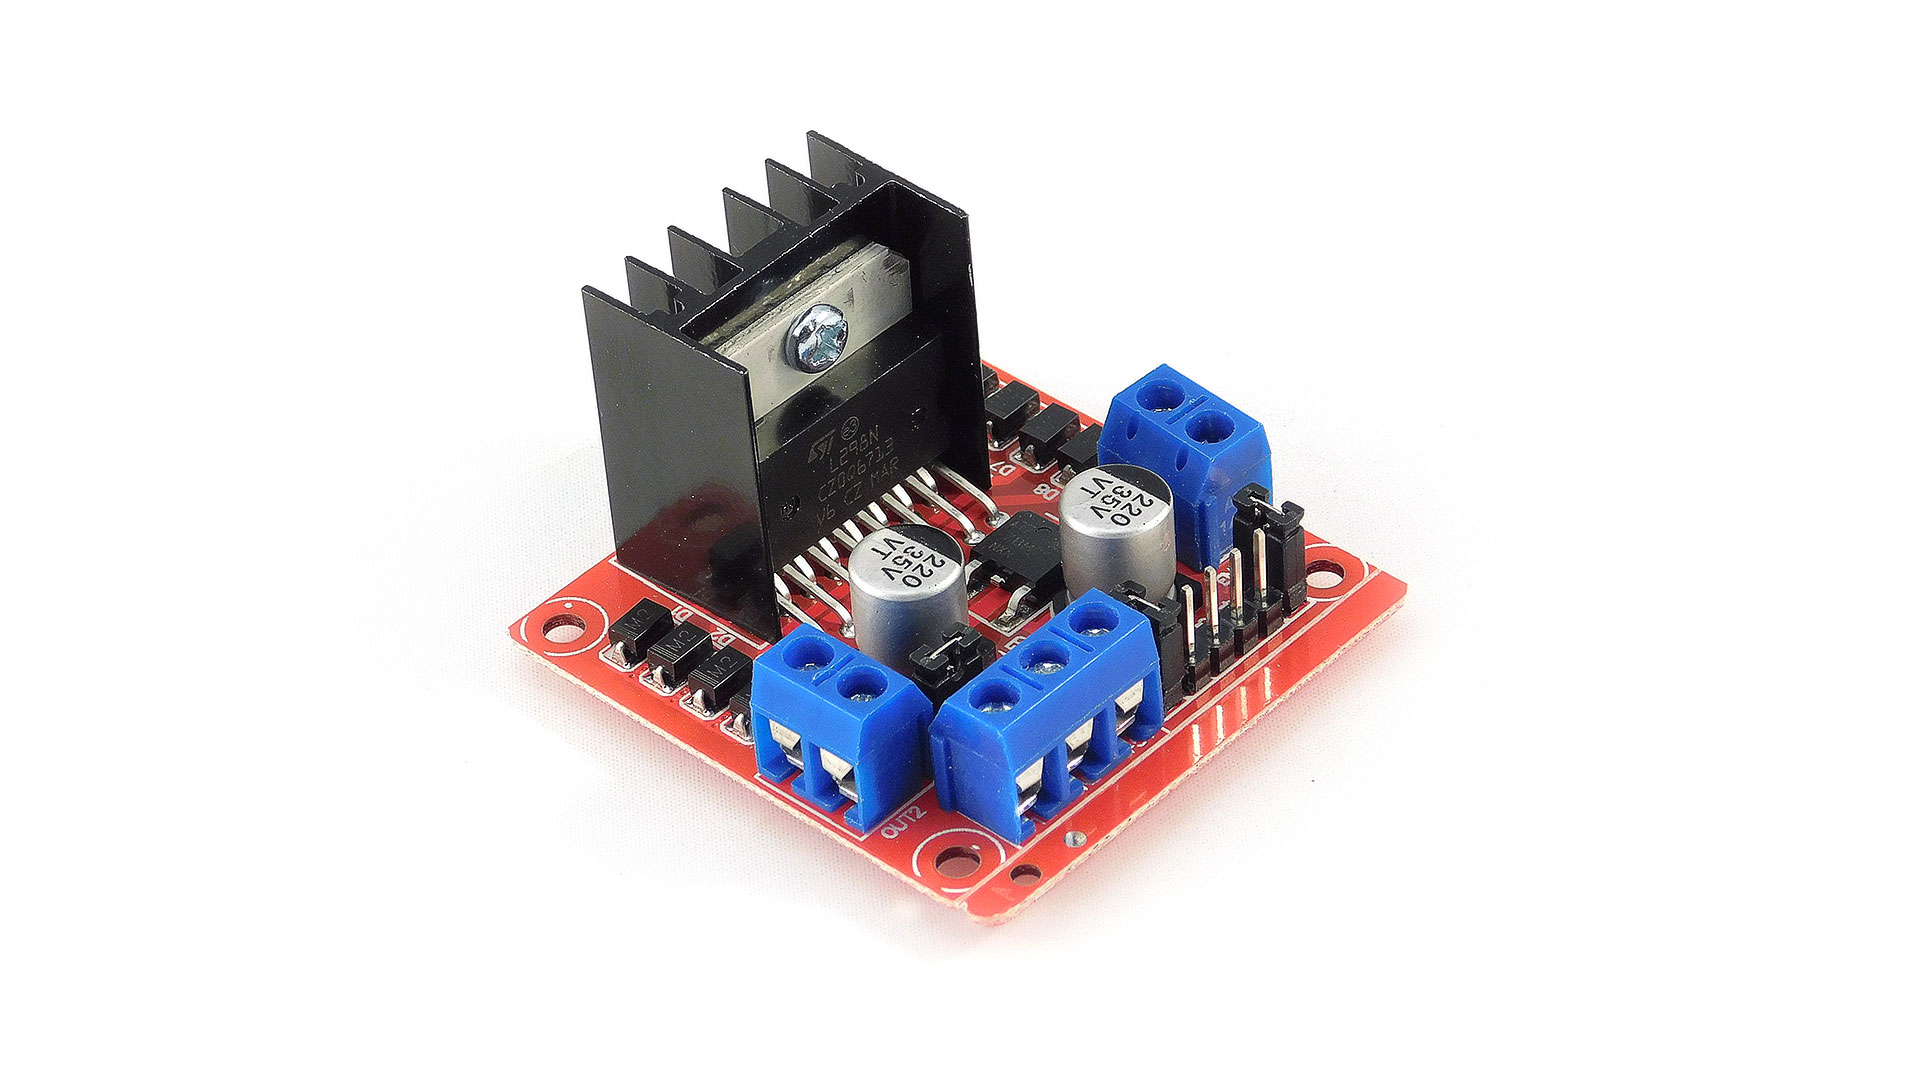
\includegraphics[scale=0.2]{praca_dyplomowa/figures/L298N.JPG}
    \caption{Sterownik silników DC L298N}
    \texttt{Źródło: botland.com.pl}
    \label{fig:L298N}
\end{figure}

\subsection{Wyświetlacz dotykowy}
Do konstrukcji został dołączony mini komputer Raspberry Pi 4 wraz z dotykowym wyświtlaczem LCD, które przedstawione są odpowiednio na zdjęciach \ref{fig:rpi4} i \ref{fig:rpidisp1}. Komunikuje się on z mikrokontrolerem STM32 poprzez magistrale UART. Zastosowanie ekranu i Raspberry Pi pozwoliły uzyskać funkcjonalność zmiany parametrów algorytmu w czasie jego pracy, bez każdorazowej kompilacji nowego programu. Zapotrzebowanie prądowo minikomputera to maksymalnie 3A, natomiast ekranu około 0,5A co łącznie daje około 17,5 W potrzebnej mocy. 

\begin{figure}
    \centering
    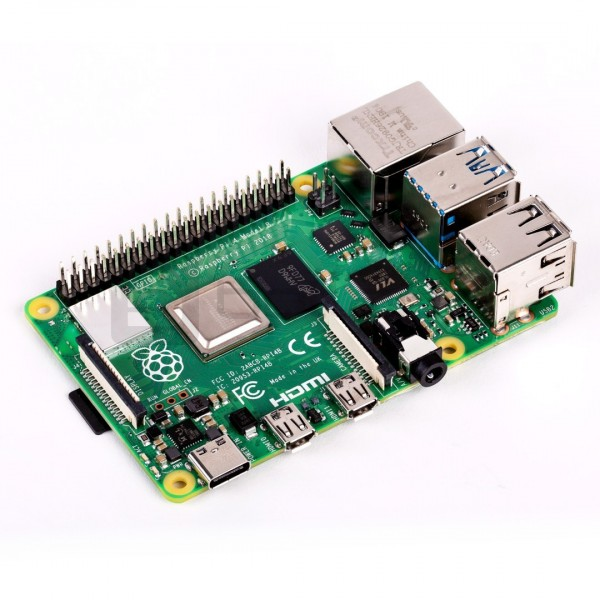
\includegraphics[scale=0.6]{praca_dyplomowa/figures/rpi4.jpg}
    \caption{Raspberry Pi 4 model B}
    \texttt{Źródło: botland.pl}
    \label{fig:rpi4}
\end{figure}

\begin{figure}
    \centering
    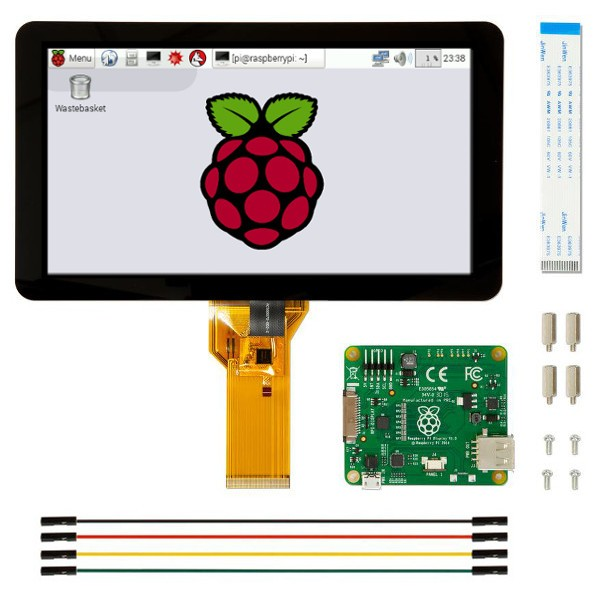
\includegraphics[scale=0.5]{praca_dyplomowa/figures/rpidisplay1.jpg}
    \caption{Dotykowy wyświetlacz Raspberry Pi}
    \texttt{Źródło: botland.pl}
    \label{fig:rpidisp1}
\end{figure}


\subsection{Zasilacz}
Do zasilania wszystkich podzespołów został użyty zasilacz komputerowy ATX o maksymalnej mocy 400W jak na rysunku \ref{fig:zasilacz}. Zaletą tego rozwiązania jest zapewnienie potrzebnych różnych napięć zasilania, bez potrzeby stosowania dodatkowych przetwornic. Zasilacz został umocowany do ramy przy pomocy samodzielnie zaprojektowanego i wydrukowanemu uchwytu.

\begin{figure}
    \centering
    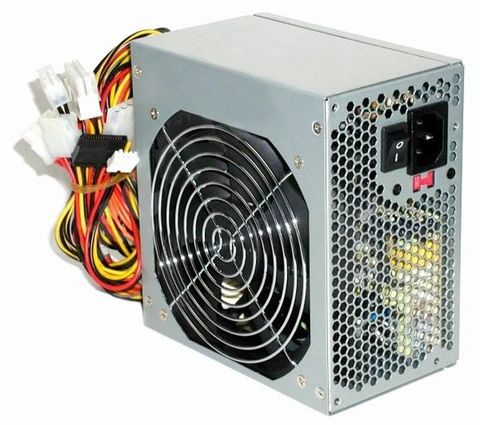
\includegraphics[scale=0.8]{praca_dyplomowa/figures/zasilacz.jpg}
    \caption{Zasilacz ATX 400W}
    \texttt{Źródło: internet-chorzow.pl}
    \label{fig:zasilacz}
\end{figure}

\section{Połączenia}

W oparciu o dokumentację wszystkich podzespołów \ref{sec:czesci} został opracowany układ pomiędzy nimi. Układ został zaprojektowany tak, aby spełniać wszystkie założenia i funkcjonalności uwzględniając również warunki bezpieczeństwa takie jak: ograniczenia termiczne, napięcie zasilania.\\
Założenia i funkcjonalności:
\begin{itemize}
    \item mikrokontroler, minikomputer, układ logiczny sterownika silnika -- maksymalne napięcie zasilania 5V,
    \item sterownik silnika -- napięcie zasilania 12V,
    \item wentylator chłodzący sterownik silnika,
    \item sprzętowa eliminacja drgań styków,
    \item wspólne źródło zasilania wszystkich komponentów.
\end{itemize}
Schemat układu przedstawiony jest na rysunku \ref{fig:schemat}. Został on wykonany za pomocą programu \textit{EasyEDA} \cite{easyeda}. 


\begin{figure}
    \centering
    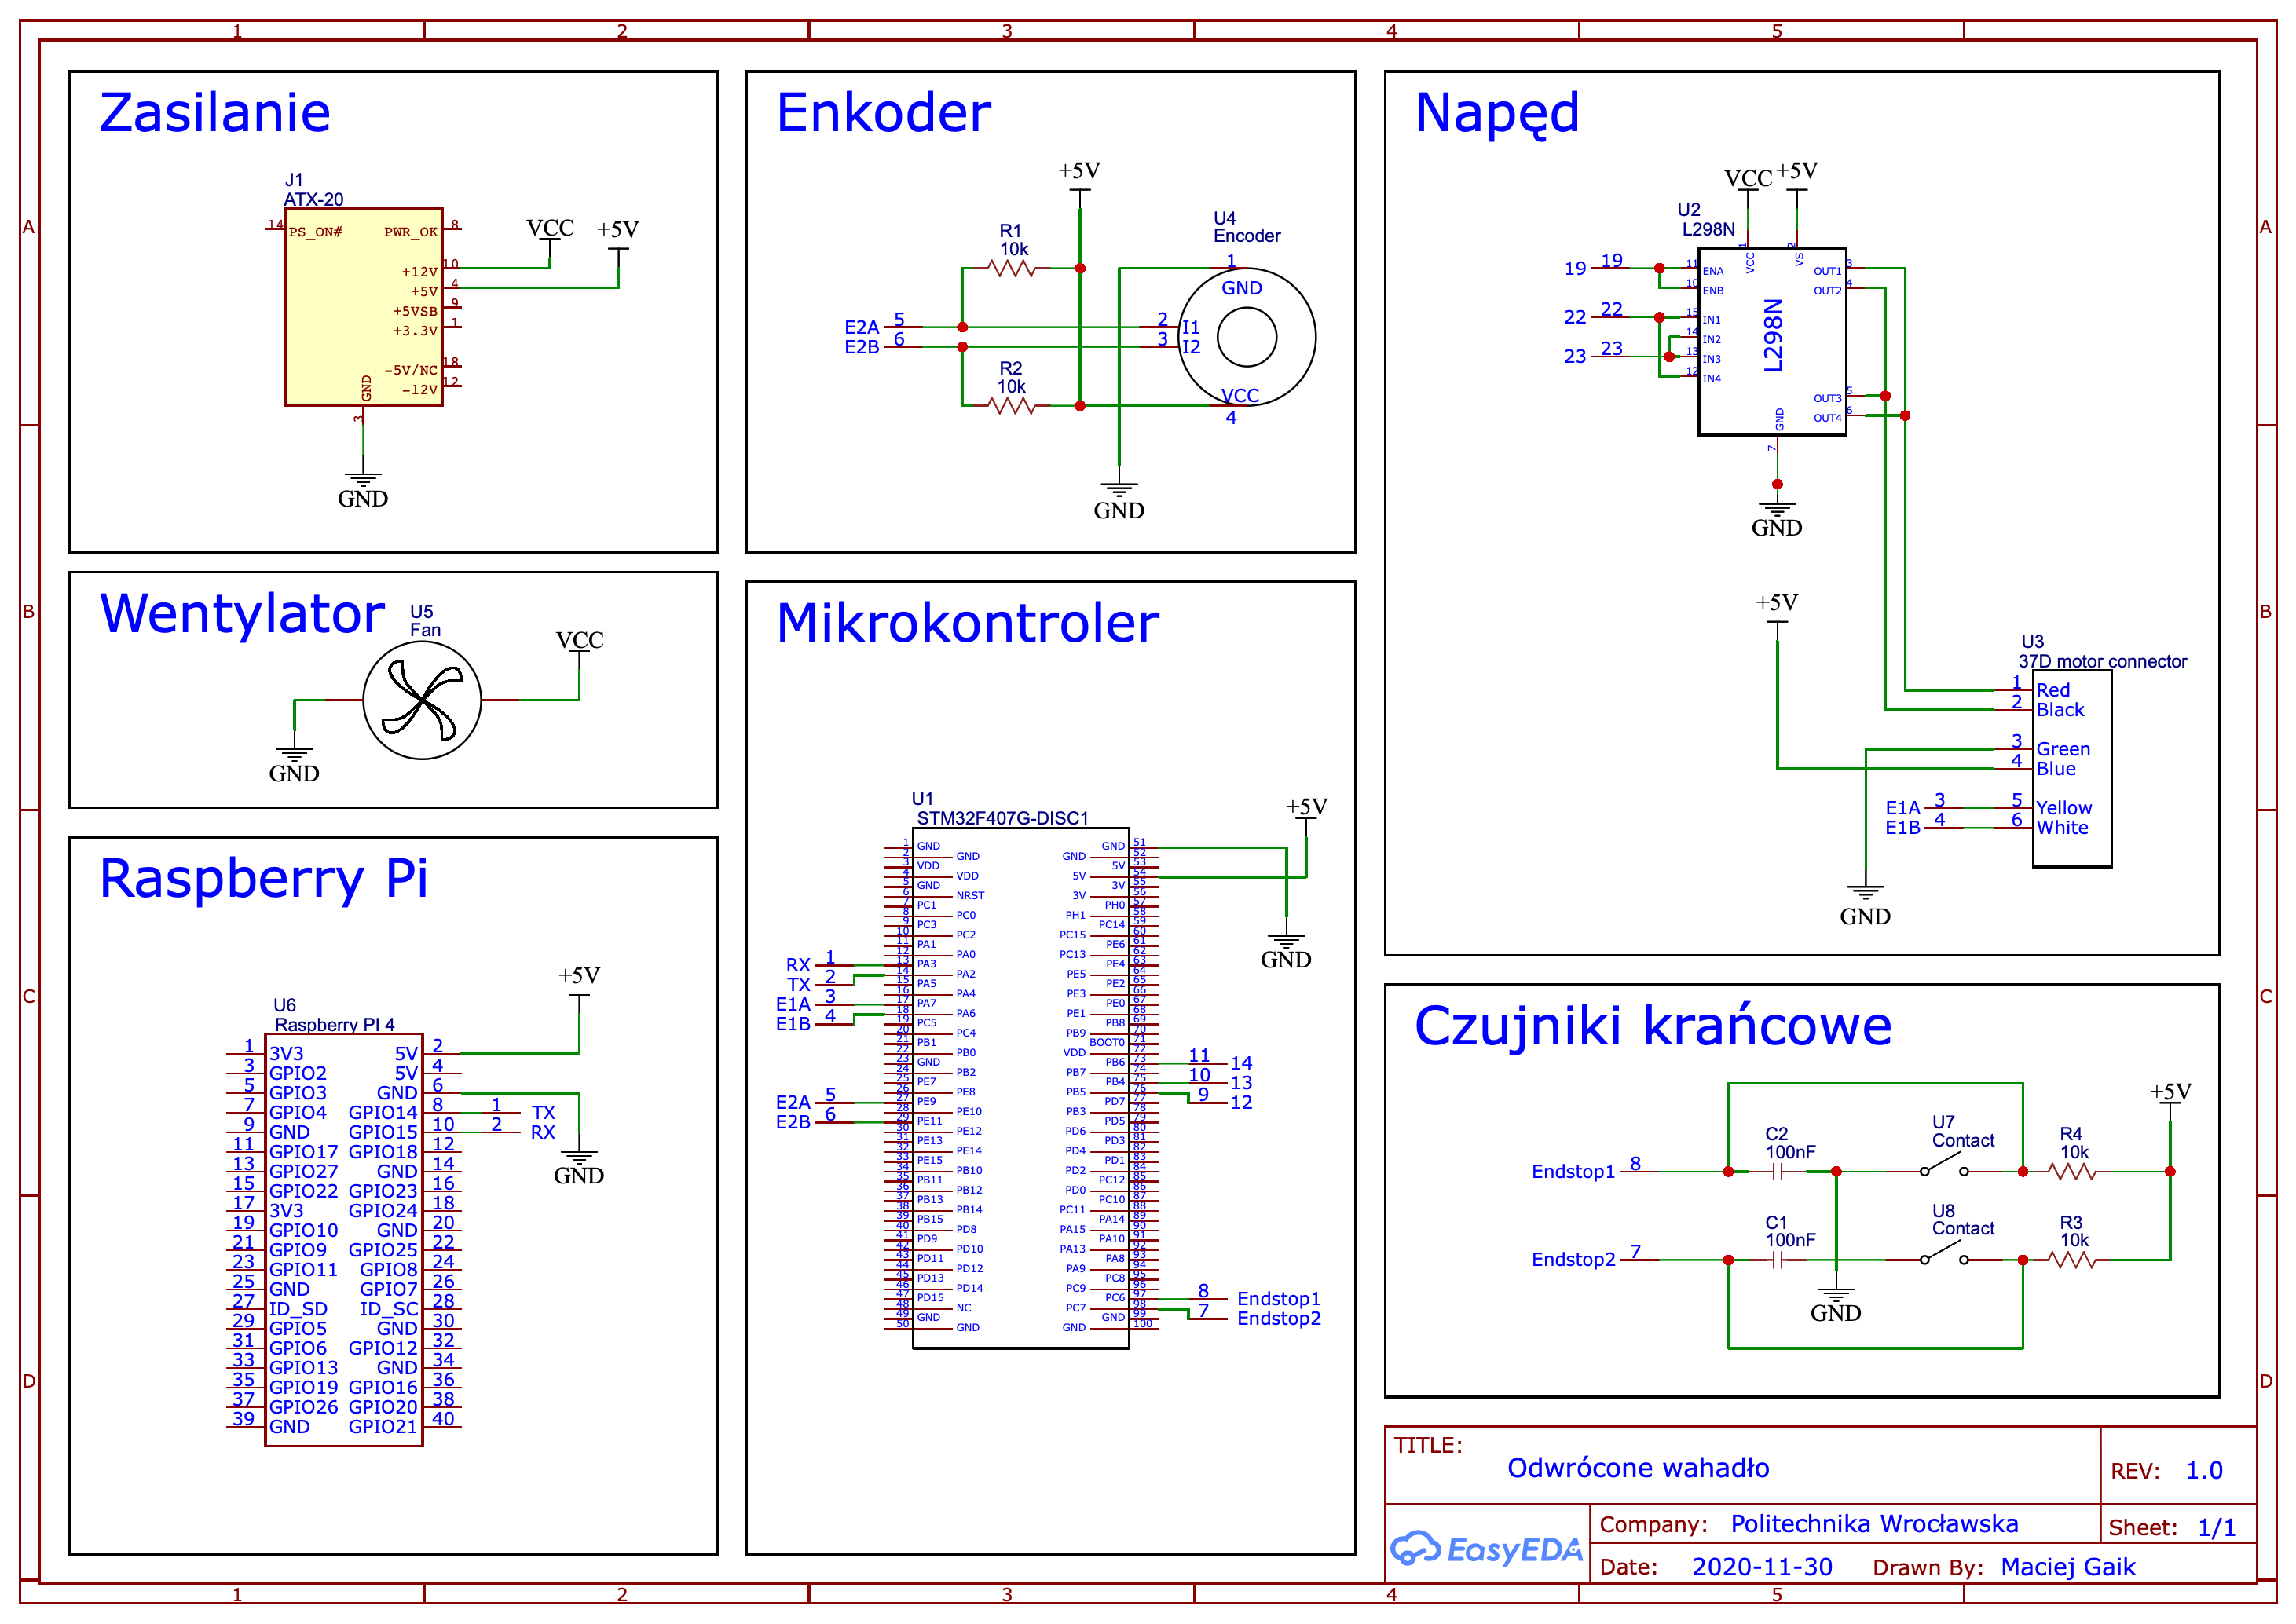
\includegraphics[rotate=-90, width=\textwidth]{praca_dyplomowa/figures/Schematic.png}
    \caption{Schemat połączeń}
    \label{fig:schemat}
\end{figure}